\subsection{Instance generation}

This section shows how the instances have been generated. Possibly adding a very schematic pseudocode of our generation algorithm.\\

This section also explains the sets of instances that are prepared for the project:\\
\begin{itemize}
	\item small-medium set: used to compare the solving time of the ILP model versus the Metaheuristics models
	\item large set: used to test the Metaheuristics models parameters over a large set of instances in order the choose the best performing setup for each model.
\end{itemize} 

\subsubsection{Instance generation}

pseudocode\\
comments\\
how feasibility is assured\\
tests on how to increment solving time, including some graphs with the Best Integer and Best Bound evolution for different variations of the same instance\\
Conclusion on how to increase the "size" of the instance without computing the solving time of the ILP model.\\

The next figures show different executions of a small modification of a problem instance. In each figure, a parameter of the problem is modified to increase the time it takes to Cplex to solve the instance problem. This gives us an idea of what parameters increase the size of the problem instance.\\

\begin{center}
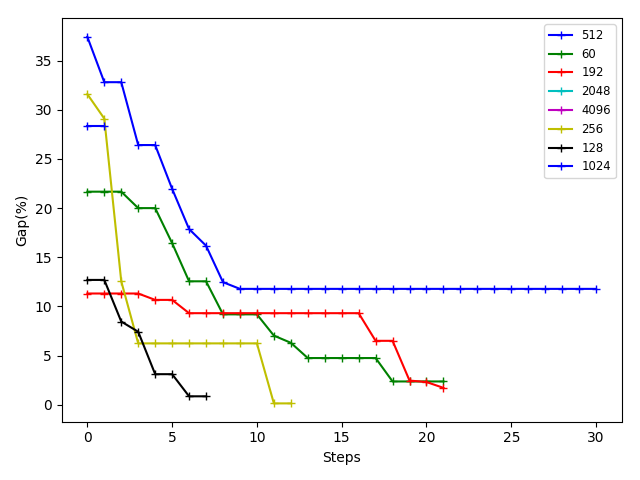
\includegraphics[width=0.5\textwidth]{./img/instances_nurses_ilp_evol.png}
\captionof{figure}{Evolution of Gap in similar problem instances with different number of nurses}
\end{center}

\begin{center}
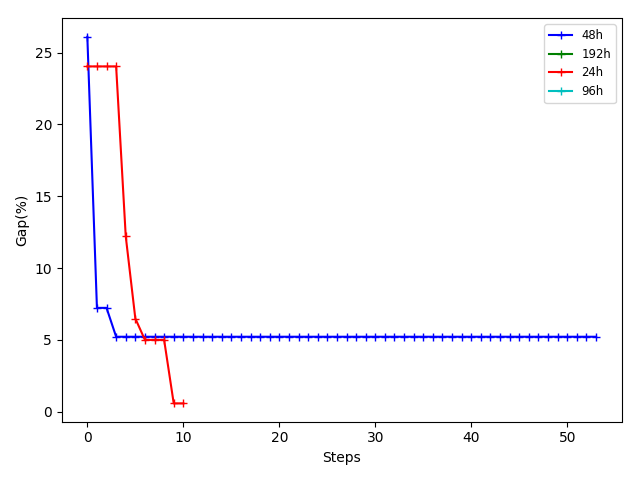
\includegraphics[width=0.5\textwidth]{./img/instances_hours_ilp_evol.png}\\[0.4cm] 
\captionof{figure}{Evolution of Gap in similar problem instances with different number of hours}
\end{center}

\begin{center}
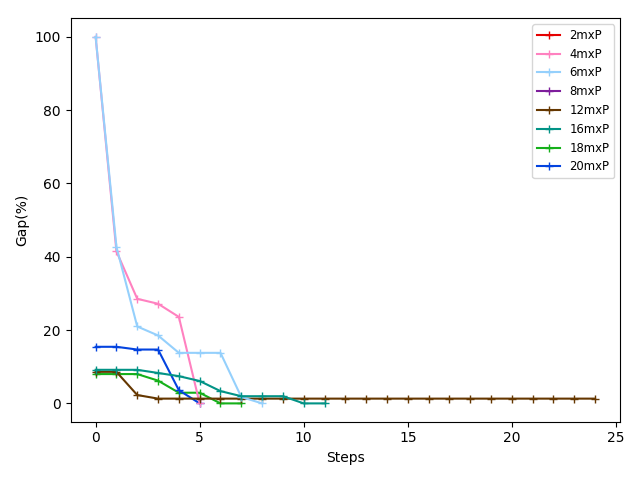
\includegraphics[width=0.5\textwidth]{./img/instances_maxpresence_ilp_evol.png}
\captionof{figure}{Evolution of Gap in similar problem instances with different values of maxPresence parameter}
\end{center}

\begin{center}
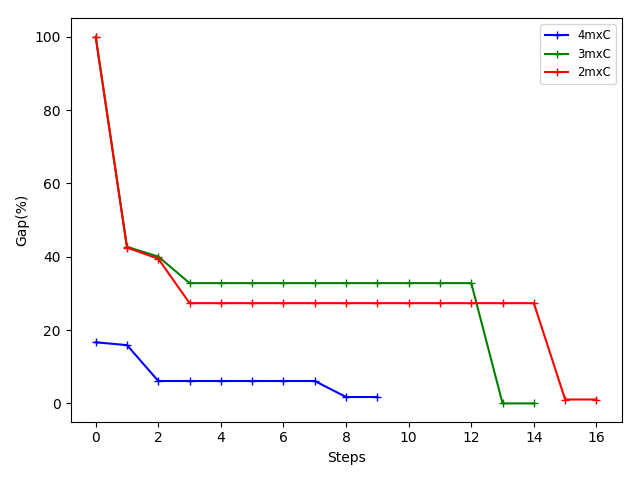
\includegraphics[width=0.5\textwidth]{./img/instances_maxconsec_ilp_evol.png}
\captionof{figure}{Evolution of Gap in similar problem instances with different values of maxConsec parameter}
\end{center}

\begin{center}
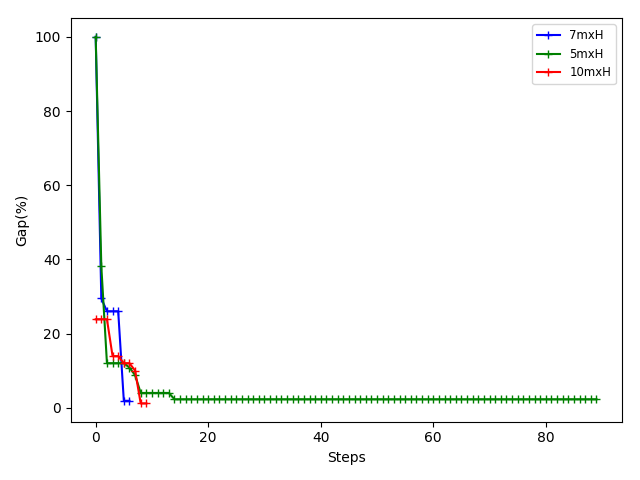
\includegraphics[width=0.5\textwidth]{./img/instances_maxhours_ilp_evol.png}
\captionof{figure}{Evolution of Gap in similar problem instances with different values of maxHours parameter}
\end{center} 

\begin{center}
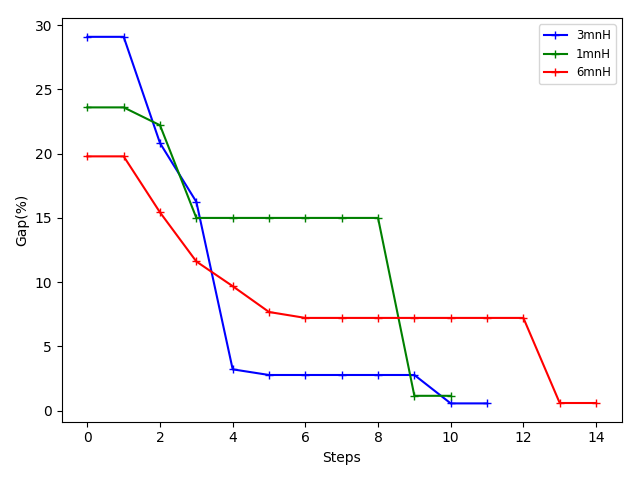
\includegraphics[width=0.5\textwidth]{./img/instances_minhours_ilp_evol.png}
\captionof{figure}{Evolution of Gap in similar problem instances with different values of minHours parameter}
\end{center}


Those small observations allow us to conclude that the number of nurses and the number of hours of a schedule are the parameteres of the problem that affect the most its solving time. Increasing the number of nurses or hours increases the size of the problem.\\
The large set of problem instances will be generated using modifications of those parameters.


\subsubsection{Medium Set}

Composition of the set, number of instances and solving times.

\subsubsection{Large Set}

Composition of the set, number of instances, solving times or another measure of the size of the problem.


\pagebreak